%ekg_7_Realisierung/Diskussion der Alternativen

\subsection{Konzeptfindung und Diskussion der Alternativen}

Dieses Unterkapitel führt die Anforderungen und die gewählten Lösungen auf, ohne diese im Detail zu erklären. Die genaue Erläuterung der verfolgten und getesteten Umsetzungen sind Inhalt der folgenden Kapitel der Realisierung. Ebenso werden hier die Lösungen aufgeführt, die sich nach dem Test als zu ineffizient oder zu aufwendig für die Anwendung erwiesen haben.

\subsubsection{Konzeptionierung}

Zur Erstellung eines Konzeptes für das EKG-Gerät wurden zunächst alle Anforderungen die sich aus dem Signal und den Produktvorstellungen ergaben, gesammelt. Hierzu zählen auch Funktionen die über die bloße Aufzeichnung eines EKGs hinausgehen.

\begin{enumerate}
\item Bandbreite der Filterschaltung: \SI{0.5}{\hertz} - \SI{160}{\hertz}
\item Abtastfrequenz: \SI{250}{\hertz} - \SI{1000}{\hertz}
\item Benötigte Verstärkung für das EKG-Signals: \SI{66}{\decibel} (= Faktor 2000)
\item Für ein Ein-Kanal-EKG muss eine Differenzbildung der Signale zwischen den beiden Ableitungspunkten durchgeführt werden
\item Die negativen Signalanteile des EKGs müssen mit einer unipolaren Versorgungsspannung übertragen werden
\item Durch Magnetfelder von umgebenden Versorgungsleitungen induzierte Störsignale (sogenanntes Netzbrummen) müssen unterdrückt werden
\item Die verwendeten aktiven elektronischen Bauteile müssen mit einer unipolaren Versorgungsspannung betrieben werden können und sollten diesen Spannungsbereich fast vollständig ausnutzen
\item Zur Anzeige des Signals soll wahlweise ein integriertes Display oder das eigene Smartphone verwendet werden
\item Die Bedienung erfolgt via Touchscreen mit einem intuitiven User-Interface
\item Als Aufnahmemodi werden ein Kurzzeit-EKG (\SI{2}{\min}) und ein Langzeit-EKG (24 Stunden) angeboten
\item Die Betriebslaufzeit muss mindestens 30 Stunden betragen
\item Die Energieversorgung erfolgt über einen Lithium-Ionen-Akku
\item Die aufgenommenen Daten werden auf einem externen Speichermedium gesichert
\item Bei einem niedrigen Akkustatus soll das Gerät den Nutzer durch einen akustischen Warnton darauf hinweisen
\end{enumerate}

Die Bandbreite wurde nach der Analyse eines künstlichen Testsignals (siehe Abbildung \ref{fig_Matlab EKG-Signal}) mithilfe von Matlab gewählt. Das EKG-Signal wurde aus Kosinus- und linearen Funktionen erstellt und danach durch eine Fast-Fourier-Transformation (FFT) das Frequenzspektrum (siehe Abbildung \ref{fig_Matlab Frequenzspektrum}) ermittelt. Die betragsmäßig größten Frequenzanteile reichen von \SI{0}{\hertz} bis etwa \SI{40}{\hertz}. Da jedoch gerade die hochfrequenten Anteile des Signals für die Ausformung der charakteristischen QRS-Zacken verantwortlich sind, wurde die Grenzfrequenz der Tiefpassfilterung auf \SI{160}{\hertz} gesetzt. Der Gleichanteil des Signals wird mit einem Hochpass abgetrennt und das Wechselsignal auf ein DC-Potenzial von etwa \SI{1,5}{\volt} überlagert. Dadurch dass die Filterschaltung auf ein Gleichspannungspotenzial von $\frac{V_{cc}}{2}$ angehoben wird, ist es möglich auch negative Signalanteile mit der einseitigen positiven Versorgungsspannung zu übertragen.

\begin{figure} [!h]
	%\centering
	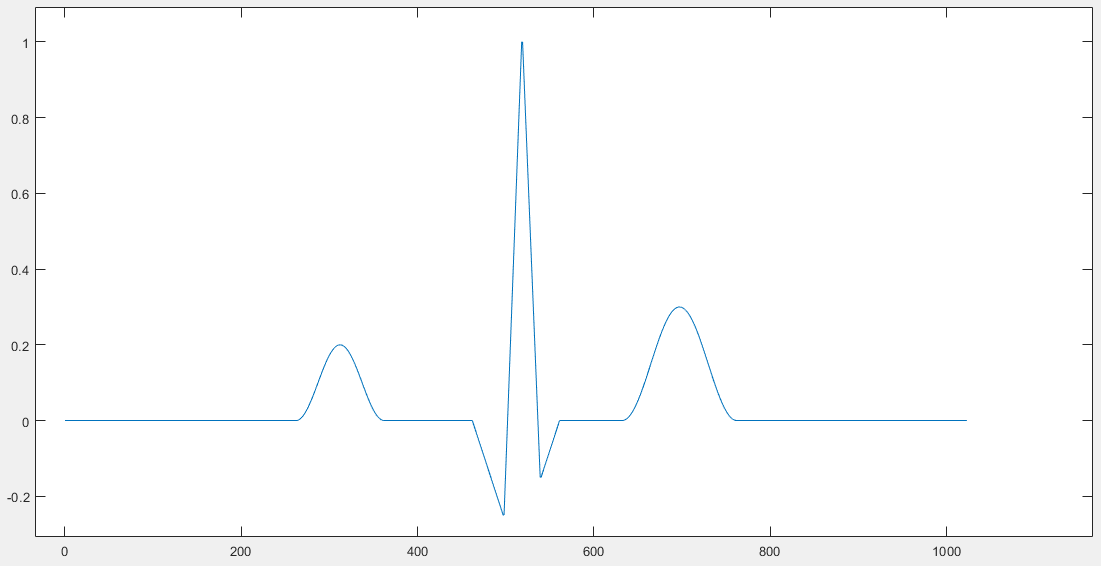
\includegraphics[width=\textwidth] {EKG_Signal.png}
	\caption{mit Matlab erstelltes künstliches EKG-Signal}
	\label{fig_Matlab EKG-Signal} 
\end{figure}

\begin{figure} [!h]
	%\centering
	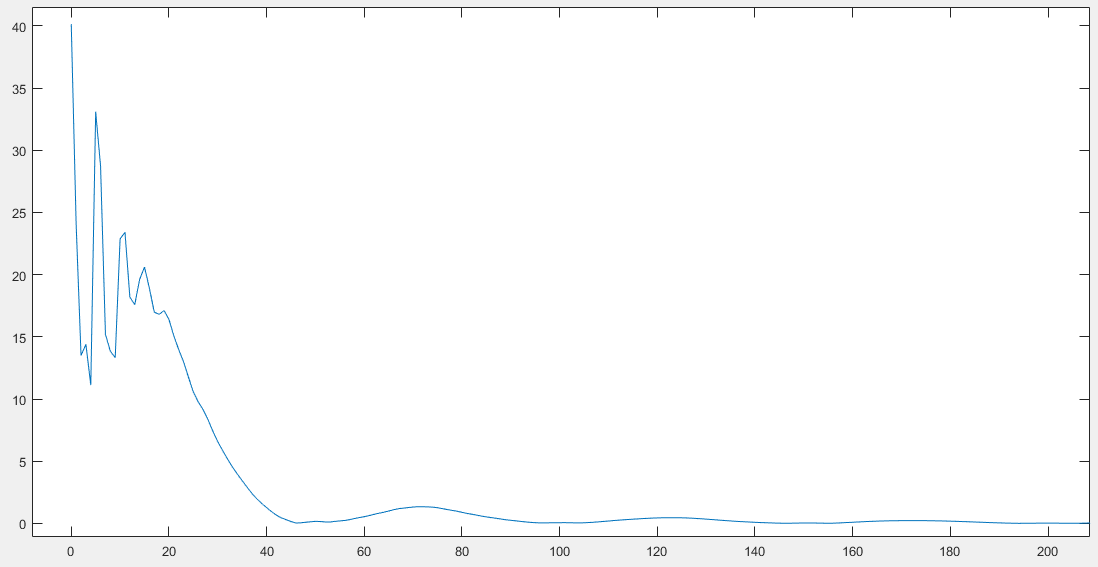
\includegraphics[width=\textwidth] {EKG_diskretes_Frequenzspektrum_Ausschnitt.png}
	\caption{Frequenzspektrum des künstlichen EKG-Signals}
	\label{fig_Matlab Frequenzspektrum} 
\end{figure}

Da das Störsignal durch Magnetfelder mit der gleichen Frequenz der Versorgungsleitungen schwingt, wird das EKG-Signal durch Kerbfilter mit einer Sperrfrequenz von \SI{50}{\hertz} gefiltert. Zur Differenzbildung der beiden Eingangskanäle wird ein Instrumentenverstärker eingesetzt. Gleichzeitig dient er zur Vorverstärkung des Signals um die Störanfälligkeit gegen elektromagnetische Felder auf dem Weg durch die Schaltung zu reduzieren. Am Ende erfolgt eine Nachverstärkung um den Arbeitsbereich und somit auch die Auflösung des ADC bestmöglich auszunutzen. Abbildung \ref{fig_Blockschaltbild Filter} zeigt die einzelnen Stufen der Filterung schematisch.

\begin{figure} [!h]
	%\centering
	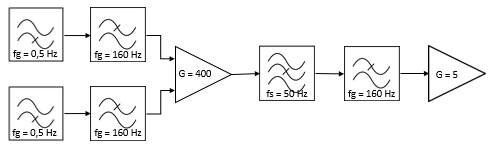
\includegraphics[width=\textwidth] {Filter Blockschaltbild.png}
	\caption{Blockschaltbild der Filterschaltung}
	\label{fig_Blockschaltbild Filter} 
\end{figure}

Wie aus Abbildung \ref{fig_Blockschaltbild} zu erkennen ist, werden zwei Versorgungsspannungen (\SI{3}{\volt}  und \SI{5}{\volt}) für die Module benötigt. Sie werden aus dem Spannungsbereich eines Lithium-Ionen-Akkus mithilfe eines LDO für \SI{3}{\volt} und eines Aufwärtswandlers für \SI{5}{\volt} erzeugt. Der Aufwärtswandler kann über einen Enable-Eingang vom Prozessor ein- oder ausgeschaltet werden, um den Stromverbrauch durch die Peripherie zu minimieren und die Akkulaufzeit zu verlängern.

Die Anzeige und Steuerung erfolgt über ein 3,2 Zoll TFT Touch Display. Es verfügt über eine serielle Schnittstelle und kommuniziert via UART mit dem Input/Ouput-Modul des Prozessors. Zur zusätzlichen Bedienung wurde ein Taster eingeplant, der zum Ein- und Ausschalten des Energiesparmodus verwendet wird. Der Buzzer dient für akustische Warnsignale bei Fehlfunktion oder einem niedrigen Ladezustand des Akkus.

Die zweite UART-Schnittstelle (Universal Asynchronous Receiver Transmitter) der CPU wird verwendet um Daten an das Bluetooth-Modul zu senden. Dieses kommuniziert dann via Bluetooth mit dem Smartphone des Benutzers, um die EKG-Daten in der App anzuzeigen.

Die Datenspeicherung erfolgt auf einer externen SD-Karte. Das Kartenmodul das zum Schreiben und Lesen der Daten verwendet wird, kommuniziert via SPI (Serial Peripheral Interface) mit dem Input/Output-Modul der CPU.


\begin{figure} [h]
	%\centering
	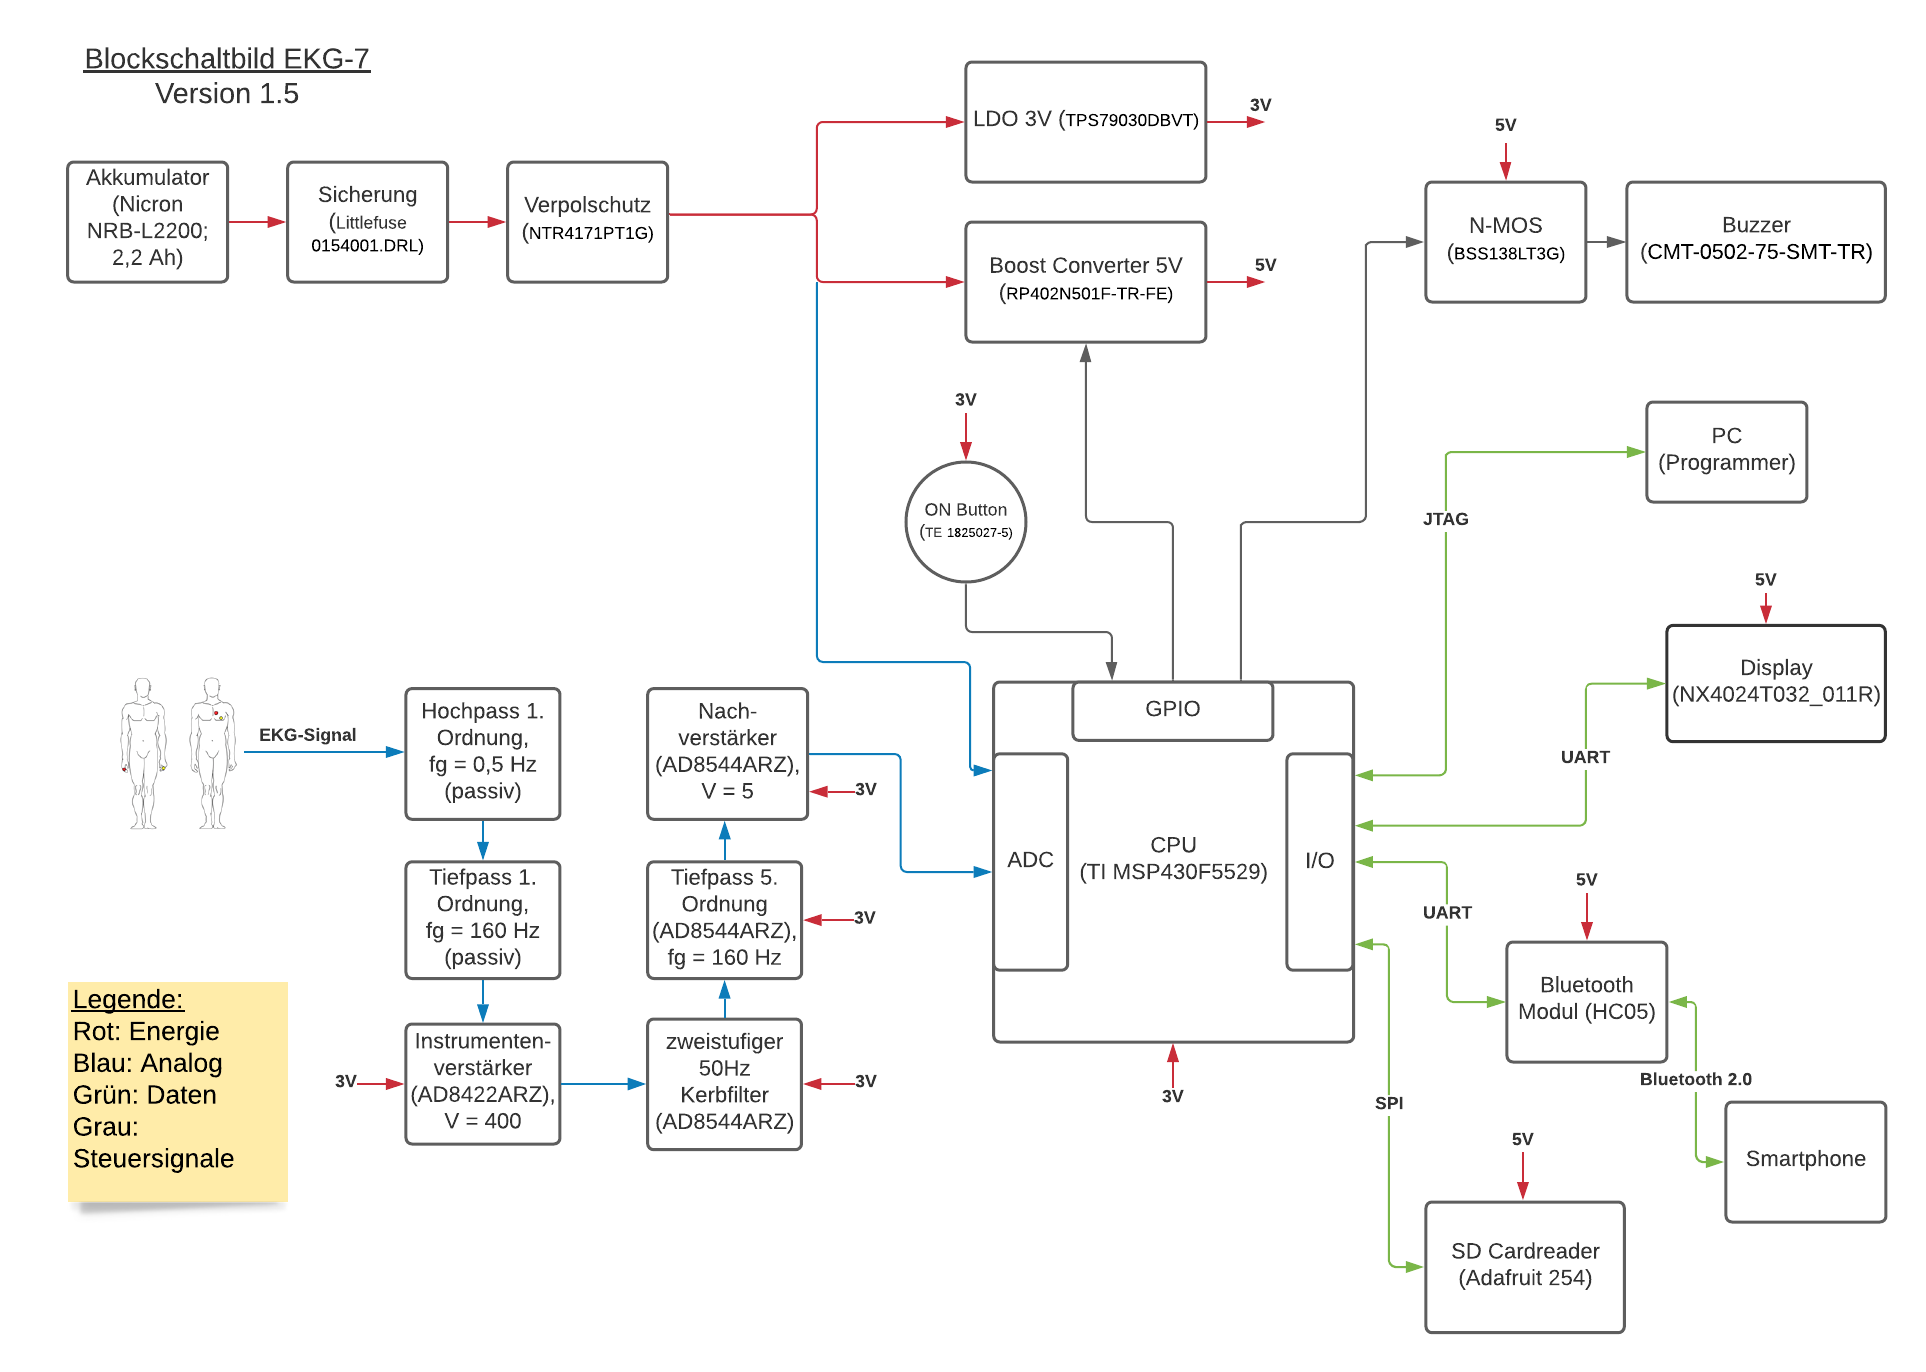
\includegraphics[width=\textwidth] {Blockschaltbild v1.5.png}
	\caption{Blockschaltbild des EKG-Geräts}
	\label{fig_Blockschaltbild} 
\end{figure}

%TODO PROJEKTGRUPPE: Konzeptionierung der jeweiligen Baugruppe; Gründe warum die jeweiligen Bauteile verwendet wurden noch hinzufügen

\subsubsection{Verwendete Software}

Für die Erstellung und Frequenzanalyse eines künstlichen EKG-Signals wurde das numerische Rechentool Matlab verwendet. Damit konnten die Grenzfrequenzen des Signals bereits ohne Labortest abgeschätzt werden. Diese Erkenntnisse wurden bei der Schaltungsentwicklung der analogen Filterschaltung mit LTSpice angewandt. Durch die Einbindung von Herstellermodellen, war die Simulation von Bauteilen möglich, ohne diese physisch zu testen. Für den Entwurf der Leiterplatine kam Altium Designer zur Anwendung. Auch hierfür bieten Hersteller Modelle für die Pinbelegung, den Footprint und 3D-Modelle an. Besonders die 3D-Modelle waren für das Gehäusedesign hilfreich um die korrekte Lage und Maße der Bauteile im Gehäuse auch optisch zu prüfen.
%TODO PROJEKTGRUPPE: weitere Software die wir verwendet haben wie Blender, Nextion Editor, CCS, Git, Android Studio etc...

\subsubsection{Verwendete Geräte}

\subsubsection{Bauteilbeschaffung und Fertigung} 

\subsubsection{Digitale Filterung}

Für die digitale Filterung des Netzbrummens wurden jeweils ein FIR- (Finite-Impuls-Response) und ein IIR- (Infinite-Impuls-Response) Filter als Bandsperren mit einer Sperrfrequenz von \SI{50} {\hertz} entworfen. Hierfür wurden die Filterkoeffizienten mit Matlab erzeugt und danach in C als eigenständige Module implementiert. Die Testung erfolgte auf dem Launchpad des MSP430 mit harmonischen Schwingungen zwischen \SI{1}{\hertz} und \SI{200}{\hertz}, einem künstlichen EKG-Signal (beides mit einer Signalquelle erzeugt) und einem echtem EKG-Signal. 

Der FIR-Filter verfügt zwar über einen linearen Phasenverlauf, erwies sich aber bei den Tests schnell als zu rechenintensiv, für die Anwendung auf dem verwendeten Prozessor. Mit ihm wurde bei einer Abtastfrequenz von \SI{250}{\hertz} lediglich eine Dämpfung von \SI{3}{\decibel} bis \SI{6}{\decibel} erreicht.

Der IIR-Filter zeigte sich im Test mit verschiedenen harmonischen Schwingungen als sehr effizient mit einer maximalen Dämpfung von \SI{150}{\decibel} bei geringem Rechenaufwand. Jedoch führte er in der Anwendung bei einem echten EKG-Signal zu einer Verschlechterung des Ausgangssignals, da er Schwingungen erzeugte, wie aus Abbildung \ref{fig_Test_IIR_Filter} zu erkennen ist. 

\begin{figure} [h]
	%\centering
	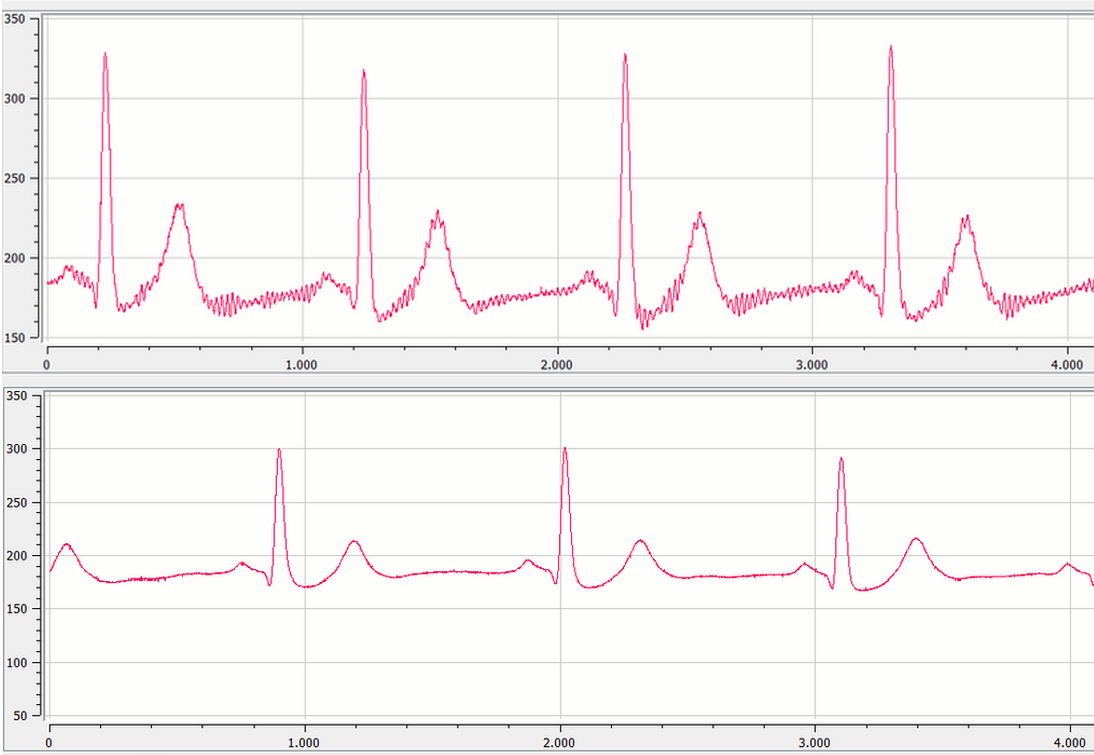
\includegraphics[width=\textwidth] {Test IIR Filter.png}
	\caption{oben: EKG-Signal mit durch IIR-Filter erzeugtes Störsignal; unten: EKG-Signal ohne IIR-Filterung}
	\label{fig_Test_IIR_Filter} 
\end{figure}
%TODO Anhang für FIR und IIR Filter



%TODO PROJEKTGRUPPE: weitere alternative Konzepte die wir ausprobiert oder in Betracht gezogen haben (zb. PMIC)